\documentclass{beamer}

\usepackage{amssymb}
\usepackage{epsfig,shadow}
\usepackage{beamerthemeshadow}

\beamertemplatetransparentcovereddynamic
\setbeamertemplate{navigation symbols}{}

%%%%%%%%%%%%%%
% Title page %
%%%%%%%%%%%%%%%%%%%%%%%%%%%%%%%%%%%%%%%%%%%%%%%%%%%%%%%%%%%%%%%%%%%%%%%%%%%%%%%

\title[OAR2]{
    OAR2\\
    An open source resource manager for large clusters
}
\author[LIG-ID]{
    {\bf LIG-ID}\\
    {\small Nicolas.Capit@imag.fr Olivier.Richard@imag.fr
            Yiannis.Georgiou@imag.fr}
}

\institute{
    \begin{center}
        \includegraphics[scale=0.4]{src/img/oar_logo.png}
    \end{center}
    {\bf http://oar.imag.fr/}
}
\date{{\tiny \today}}

\begin{document}

\frame[plain]{\titlepage}

%%%%%%%%%%%%%%%%%%%%%
% Table of contents %
%%%%%%%%%%%%%%%%%%%%%%%%%%%%%%%%%%%%%%%%%%%%%%%%%%%%%%%%%%%%%%%%%%%%%%%%%%%%%%%

\frame{
    \frametitle{Part I: Production versions}
    \tableofcontents[pausesections,part=1]
}

\frame{
    \frametitle{Part II: Research}
    \tableofcontents[part=2]
}

%%%%%%%%%%%%%%
% First part %
%%%%%%%%%%%%%%%%%%%%%%%%%%%%%%%%%%%%%%%%%%%%%%%%%%%%%%%%%%%%%%%%%%%%%%%%%%%%%%%
\part{Production versions}
\frame{\partpage}

\section{Introduction}
        \frame{
            \frametitle{What is OAR designed for}
            \begin{itemize}
                \item TOTO
                \pause
                \item TITI
                \pause
                \item TITI
            \end{itemize}
        }
        \frame{
            \frametitle{Goals}
            \begin{itemize}
                \item TOTO2
            \end{itemize}
        }
        \frame{
            \frametitle{OAR2 key words}
            \begin{itemize}
                \item TOTO
            \end{itemize}
        }

\section{Strong concepts}
    \subsection{Modules around a database}
        \frame{
            \frametitle{OAR}
            \begin{itemize}
                \item TOTO
            \end{itemize}
        }
    \subsection{Hierarchical resources}
        \frame{
            \frametitle{OAR}
            \begin{center}
                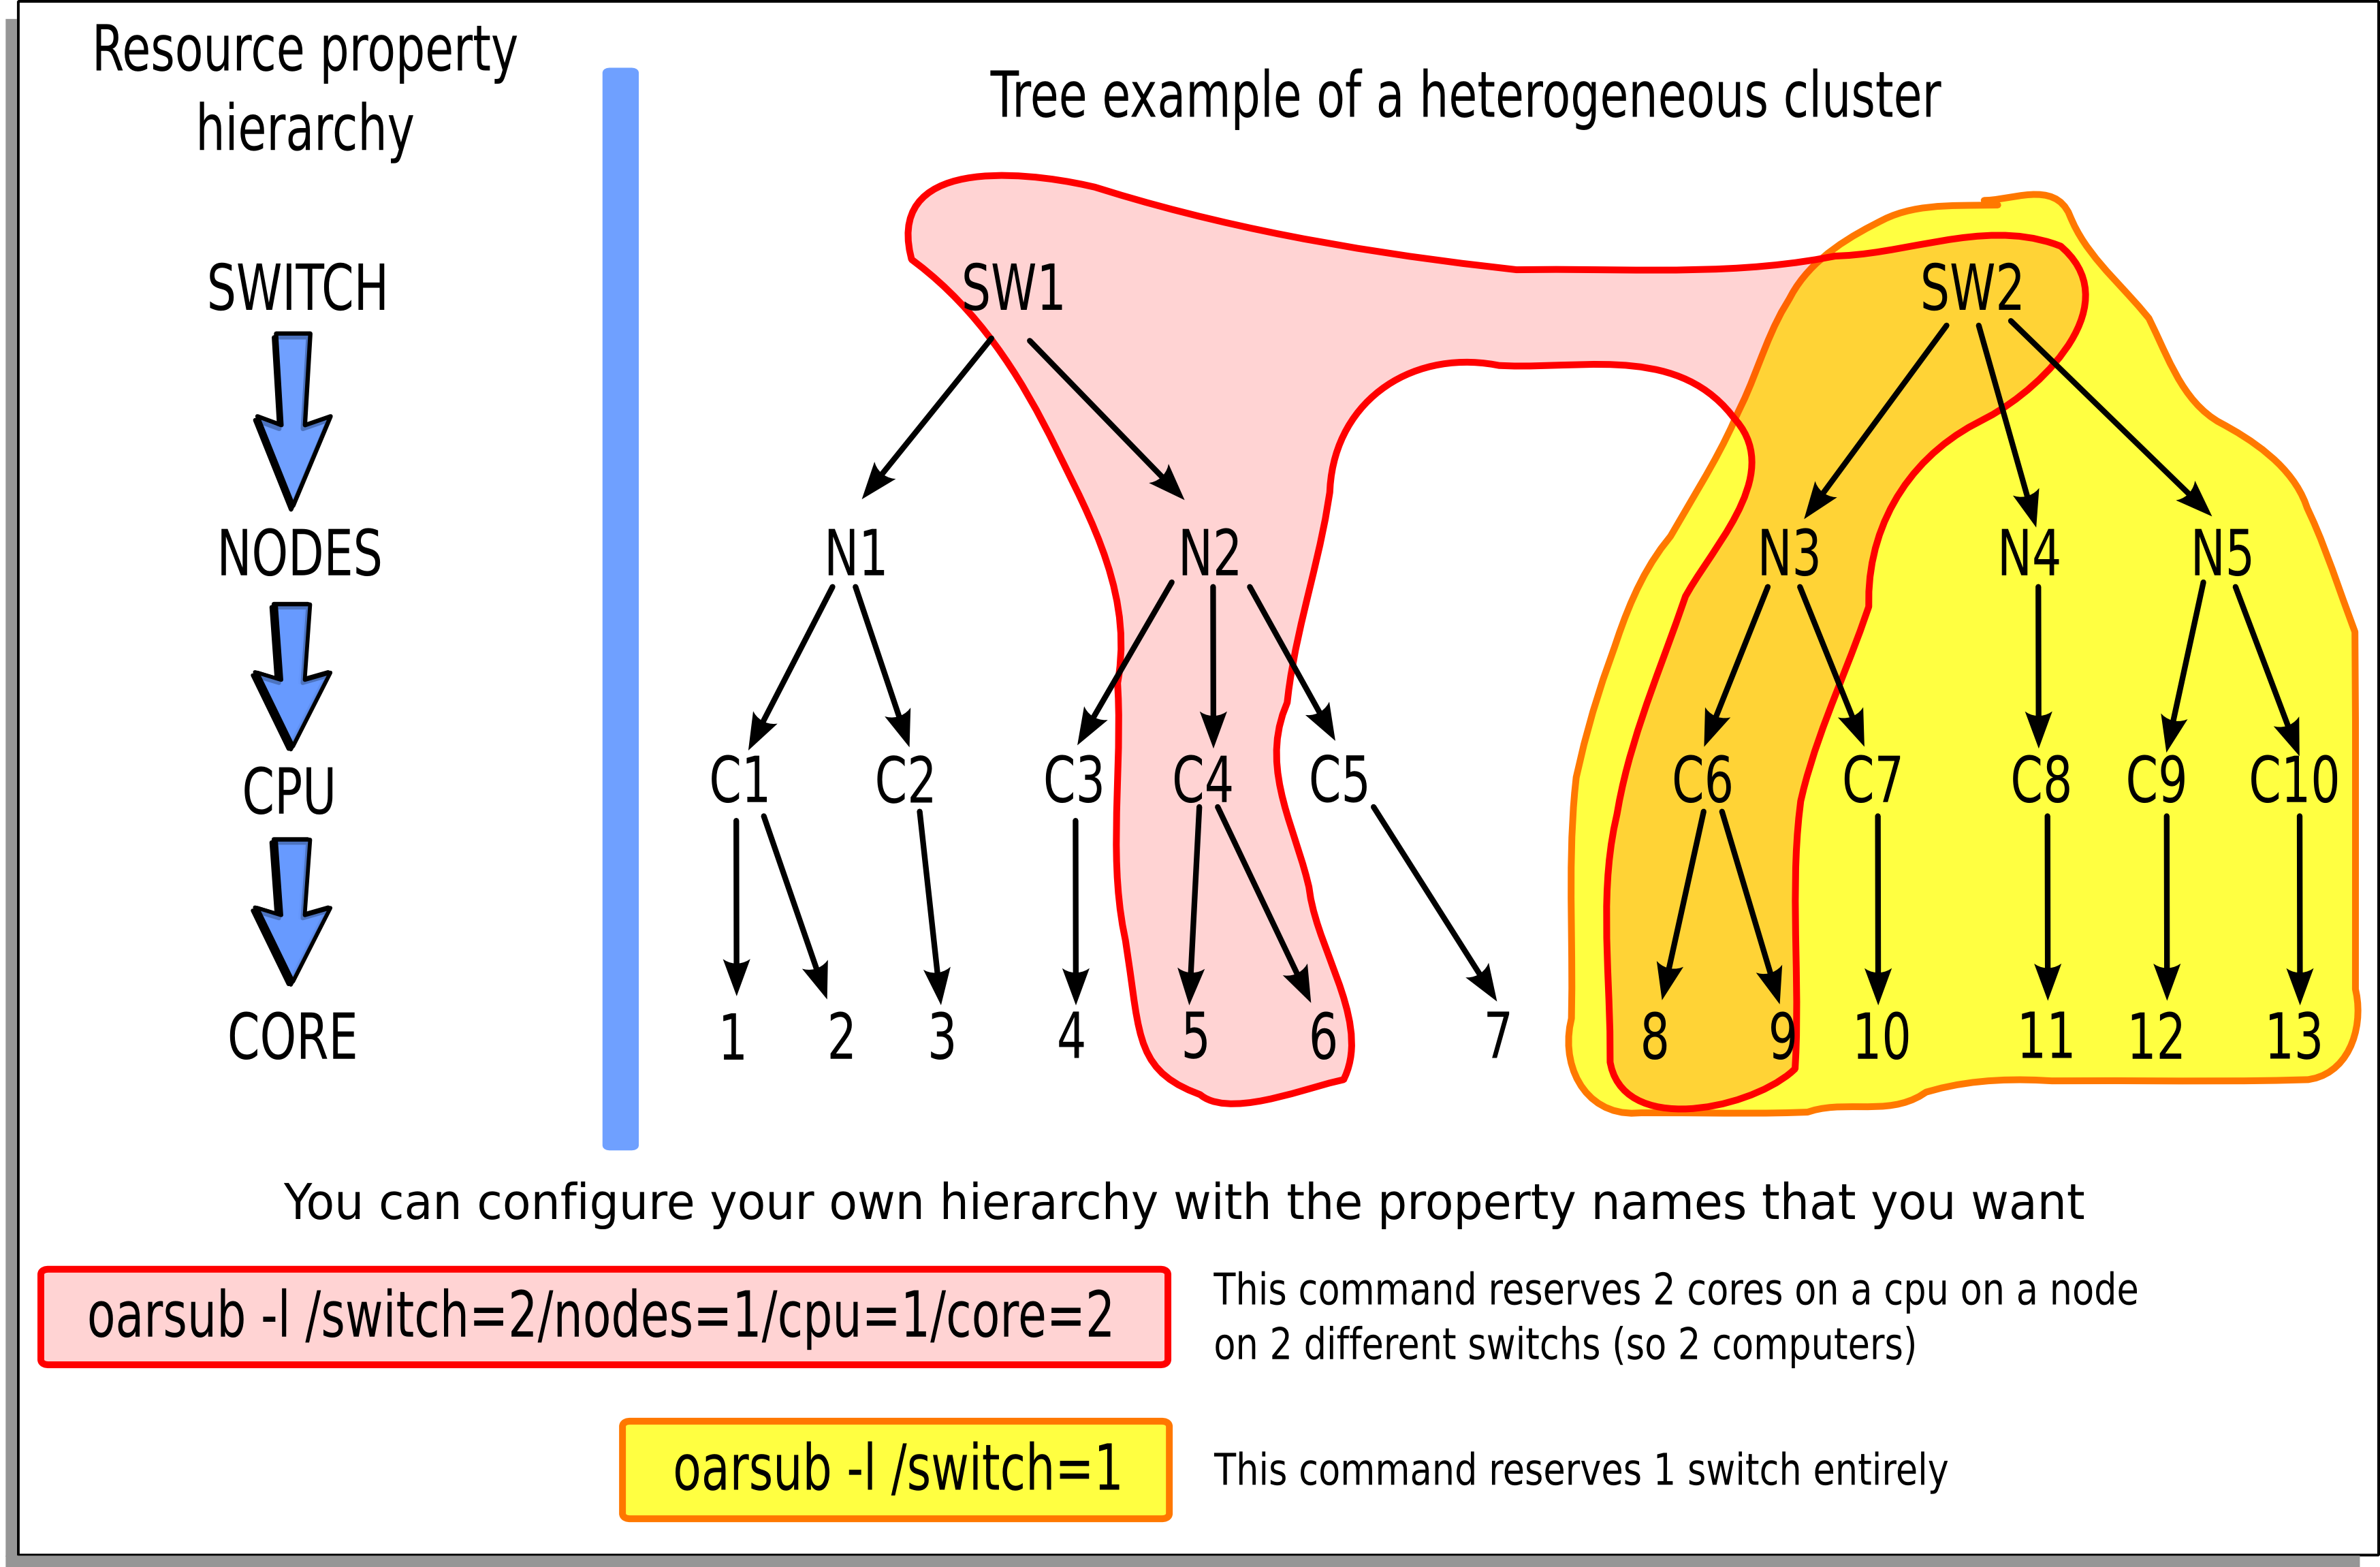
\includegraphics[height=40ex]{src/img/hierarchical_resources.png}
            \end{center}
        }
    \subsection{oarsh}
        \frame{
            \frametitle{oarsh/oarsh\_shell}
            Wrapper around the ssh command.\\
            Connect on compute nodes.
            \begin{itemize}
                \item Advantages
                \item Drawbacks
            \end{itemize}
        }
        \frame{
            \frametitle{CPUSETs}
            \begin{itemize}
                \item TOTO
            \end{itemize}
        }
        \frame{
            \frametitle{job key}
            \begin{itemize}
                \item TOTO
            \end{itemize}
        }
        \frame{
            \frametitle{job temporary user}
            \begin{itemize}
                \item TOTO
            \end{itemize}
        }
    \subsection{Scalability}
        \frame{
            \frametitle{Taktuk}
            \begin{itemize}
                \item TOTO
            \end{itemize}
        }
        \frame{
            \frametitle{Scheduling}
            \begin{itemize}
                \item Every possibilities == impossible
                \item hirearchical job resource description == make the job of the scheduler easier and so more scalable
            \end{itemize}
        }

\section{Functionalities}
    \subsection{Administrator side}
        \frame{
            \frametitle{OAR}
            \begin{itemize}
                \item TOTO4
            \end{itemize}
        }

    \subsection{User side}
        \frame{
            \frametitle{OAR}
            \begin{itemize}
                \item TOTO4
            \end{itemize}
        }


    \subsection{Simple use cases}
        \frame{
            \frametitle{OAR}
            \begin{itemize}
                \item TOTO4
            \end{itemize}
        }

    \subsection{More complex use cases}
        \frame{
            \frametitle{OAR}
            \begin{itemize}
                \item TOTO4
            \end{itemize}
        }

\section{OAR2 in action}
    \frame{
        \frametitle{OAR}
        OAR2 is ready for production and is already installed on:
        \begin{itemize}
            \item TOTO4
            \item TOTI3
        \end{itemize}
    }
    \frame{
        \frametitle{Versioning}
        The current stable branch is the 2.2.\\
        The third digit is used to bring out only bug fix released.\\
        \bigskip
        The version under development is the 2.3.\\
        \bigskip
        Other branches can be used for research oriented experimentations.\\
    }

%%%%%%%%%%%%%%%
% Second part %
%%%%%%%%%%%%%%%%%%%%%%%%%%%%%%%%%%%%%%%%%%%%%%%%%%%%%%%%%%%%%%%%%%%%%%%%%%%%%%%
\part{Research}
\frame{\partpage}

\frame{
    \frametitle{Part II: Research}
    \tableofcontents[pausesections,part=2]
}


\section{YOPYOYPOP}
\frame{
    \frametitle{First slide}
    Yop
}

\section{YEPYEPEYEP}
\frame{
    \frametitle{Second slide}
    Yep
}

\end{document}

